\section{Pursuit Domain}
\label{sec:domain}

\begin{figure*}[t]
\centering
\begin{subfigure}[t]{0.19\textwidth}
\centering
\captionsetup{width=0.9\textwidth}
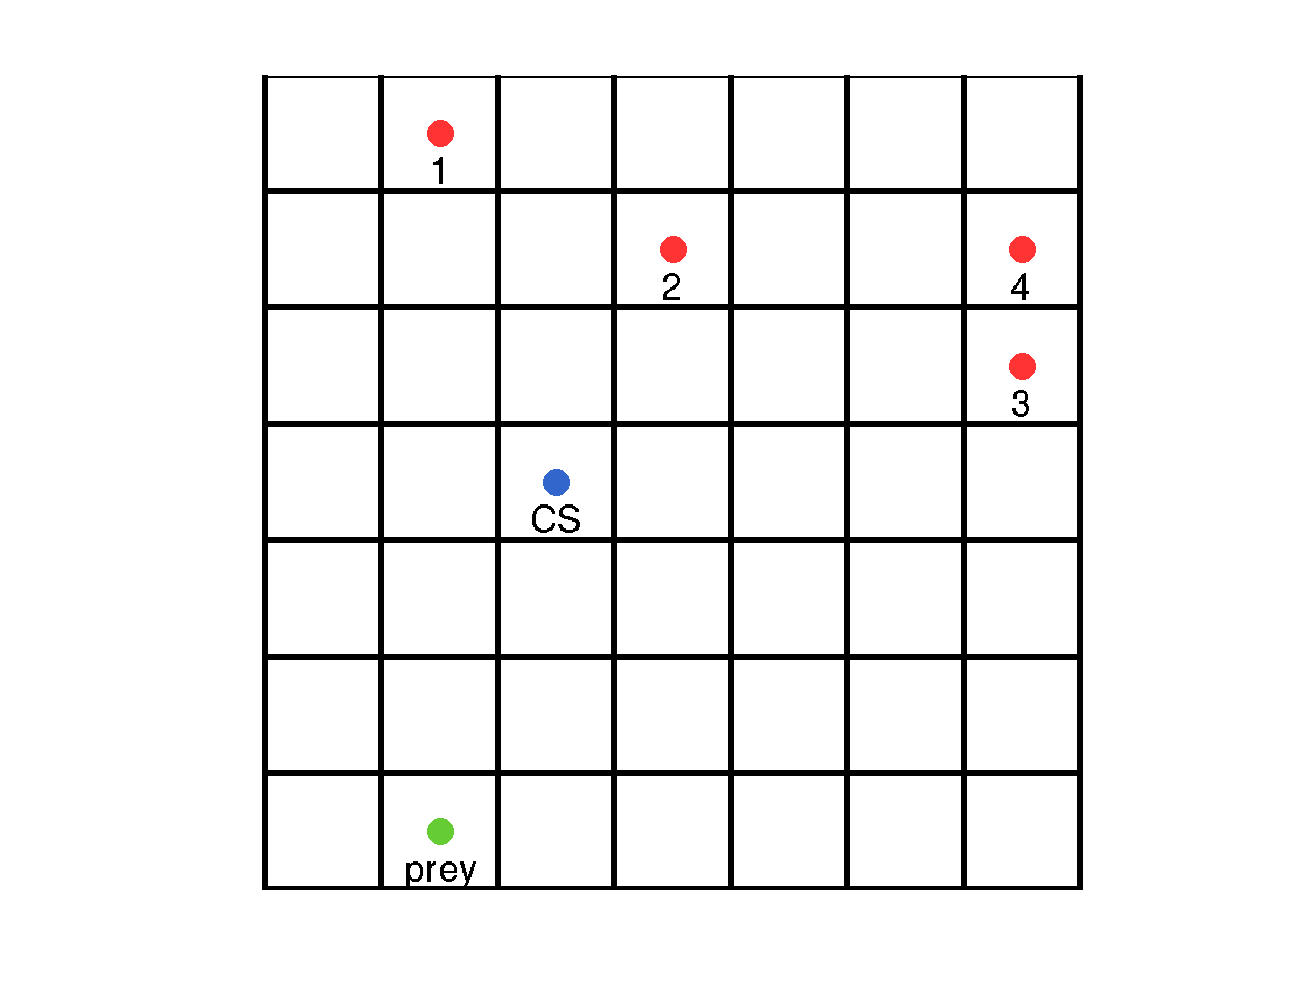
\includegraphics[trim=7cm 3cm 6cm 2cm, clip=true, width=\gridwidth\textwidth]{plots/visuals/teamConfigRandom.png}
\caption{A random position.}
\label{fig:randpos}
\end{subfigure}
\begin{subfigure}[t]{0.19\textwidth}
\centering
\captionsetup{width=0.9\textwidth}
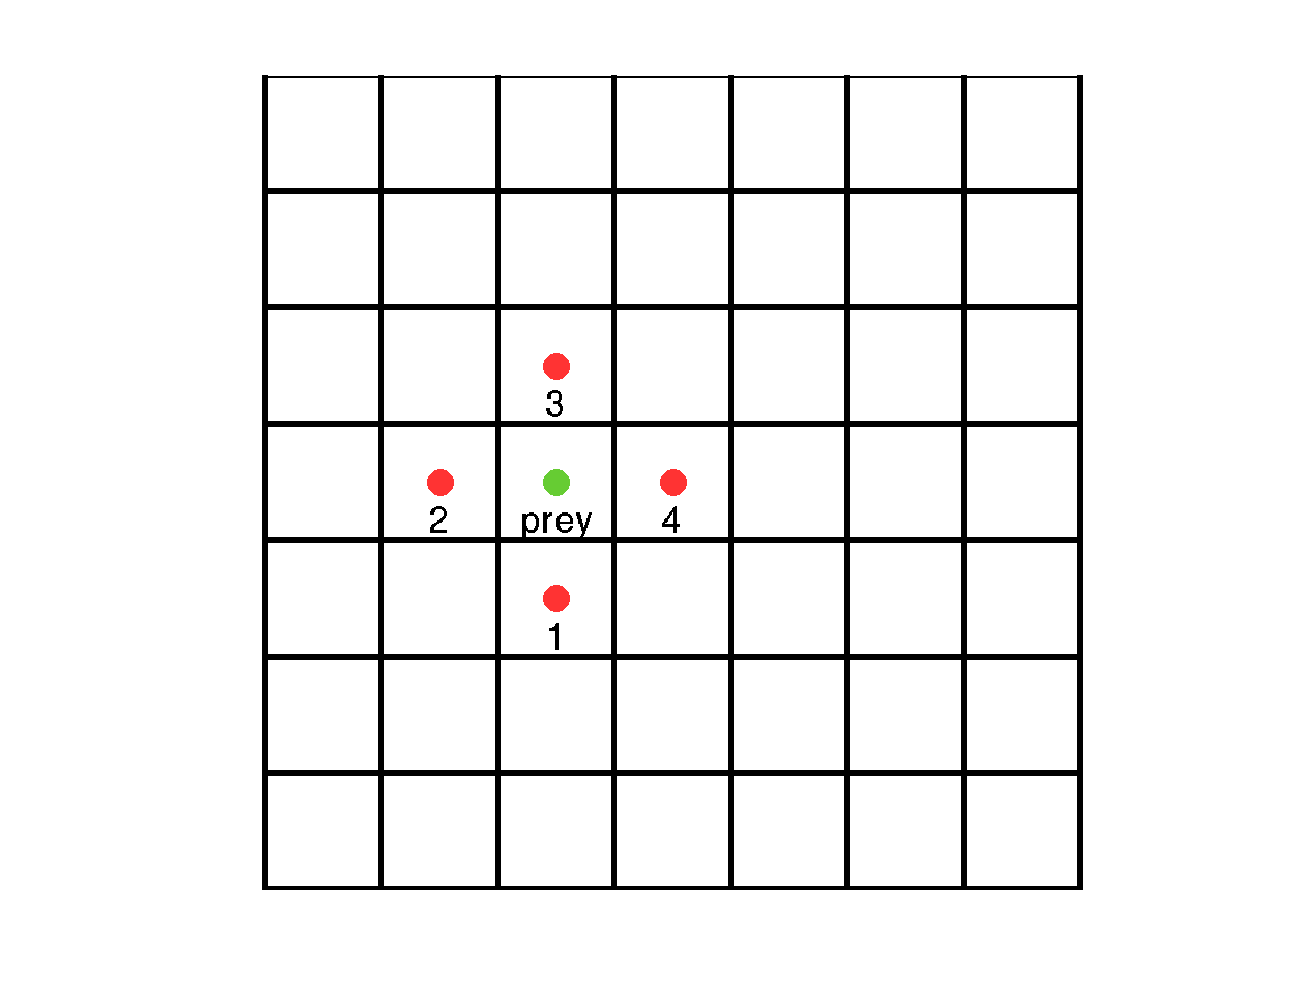
\includegraphics[trim=7cm 3cm 6cm 2cm, clip=true, width=\gridwidth\textwidth]{plots/visuals/teamConfigCapture.png}
\caption{A capture position.}    \label{fig:capturepos}
\end{subfigure}
\begin{subfigure}[t]{0.19\textwidth}
\centering
\captionsetup{width=0.9\textwidth}
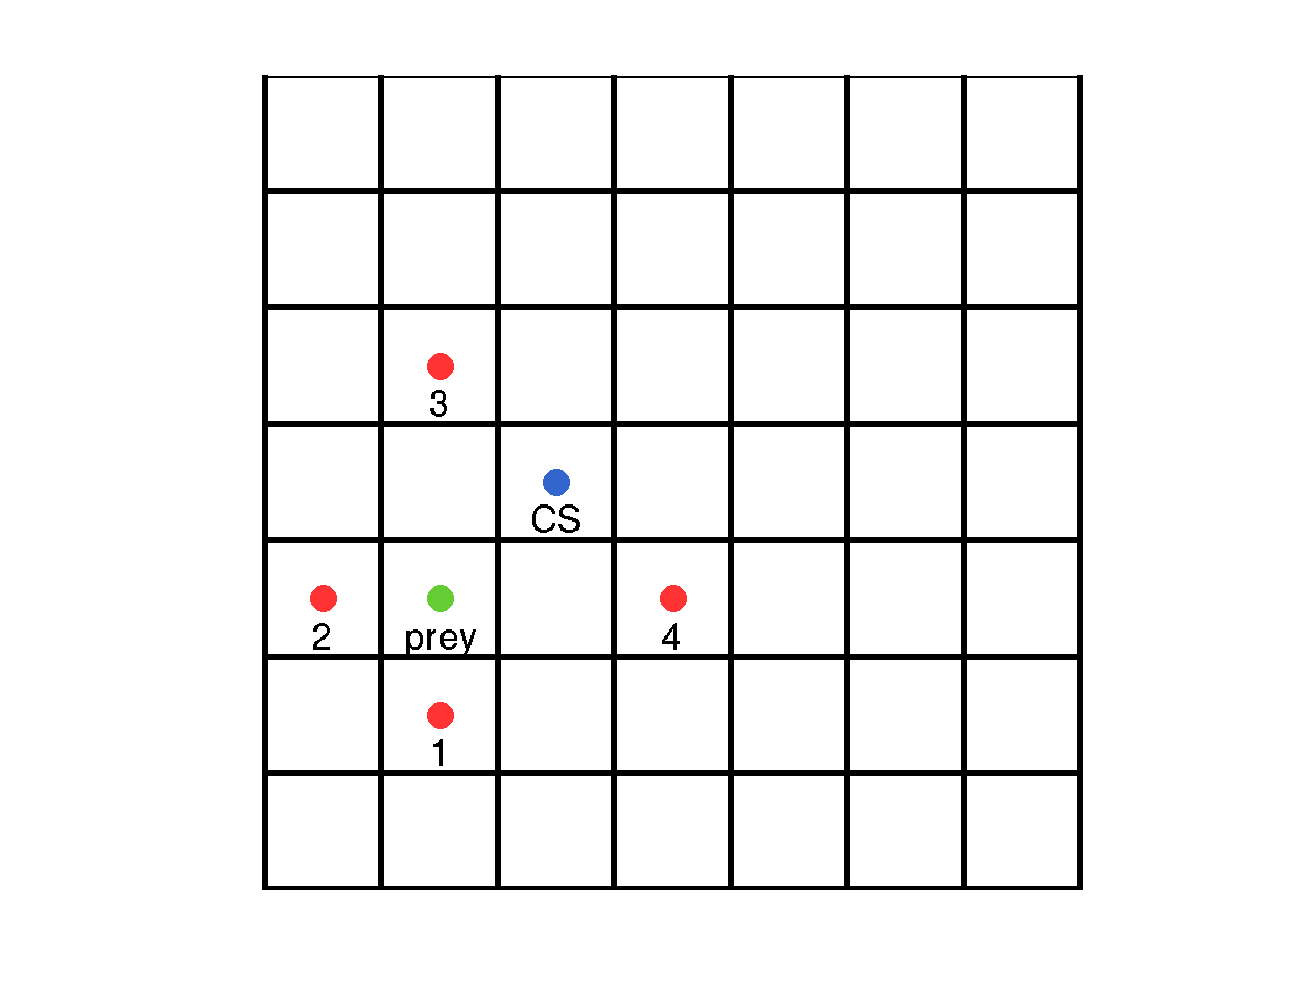
\includegraphics[trim=7cm 3cm 6cm 2cm, clip=true, width=\gridwidth\textwidth]{plots/visuals/teamConfigApproach.png}
\caption{The predators chasing the prey to the North-East.}
\label{fig:capturepos}
\end{subfigure}
\begin{subfigure}[t]{0.19\textwidth}
\centering
\captionsetup{width=0.9\textwidth}
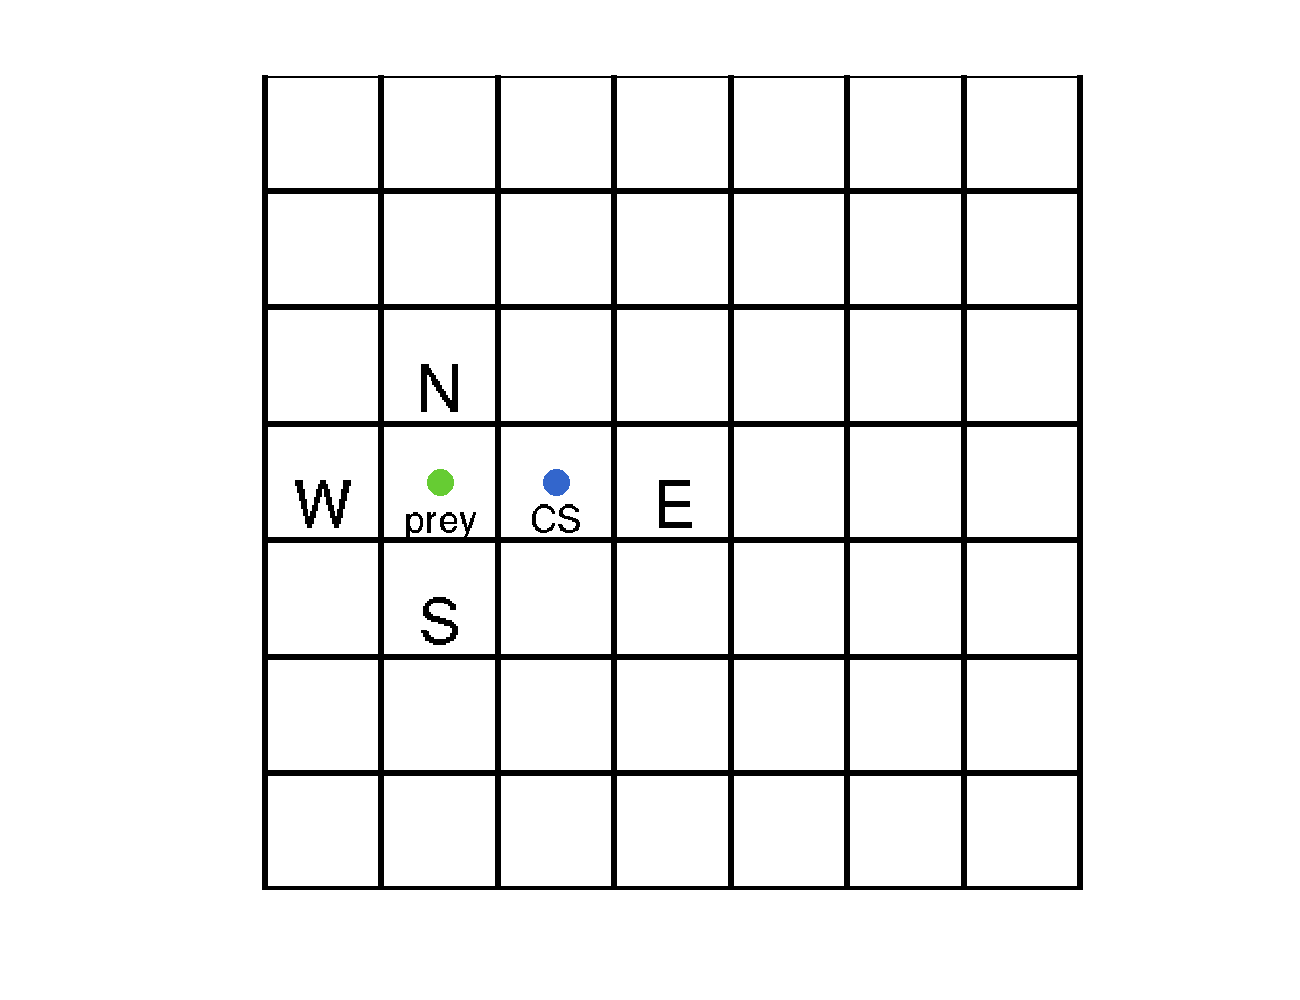
\includegraphics[trim=7cm 3cm 6cm 2cm, clip=true, width=\gridwidth\textwidth]{plots/visuals/targetStates_11.png}
\caption{States to target for each predator, chasing East.}
\label{fig:role11}
\end{subfigure}
\begin{subfigure}[t]{0.19\textwidth}
\centering
\captionsetup{width=0.9\textwidth}
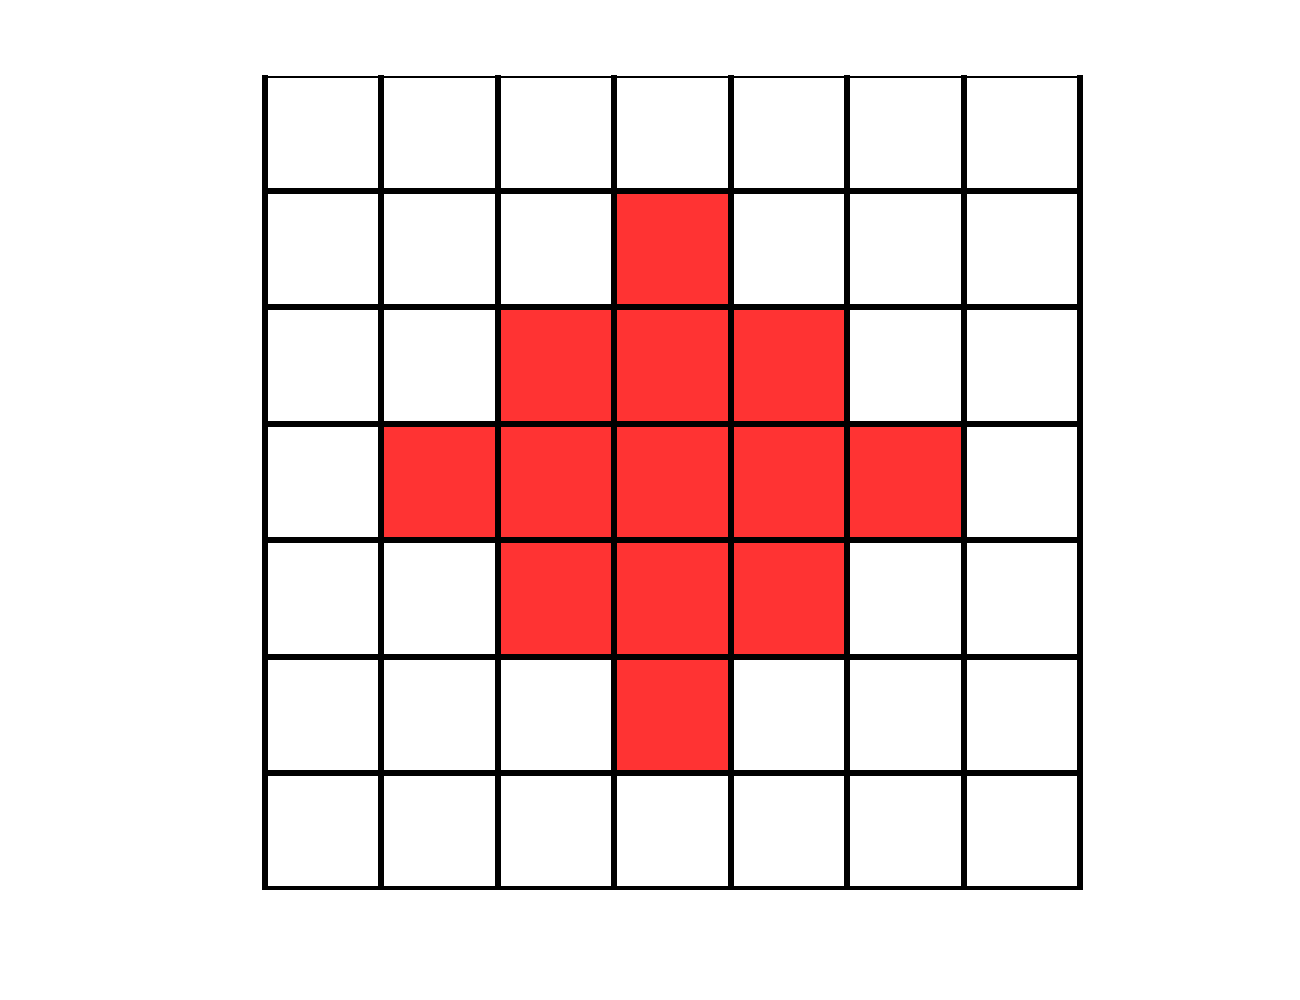
\includegraphics[trim=7cm 3cm 6cm 2cm, clip=true, width=\gridwidth\textwidth]{plots/visuals/visibleStatesMiddle.png}
\caption{States observable by a predator in position (3,3).}
\label{fig:visiblecenter}
\end{subfigure}
\caption{Illustration of the pursuit domain, the team strategy, and the partial observability. The green circle is the prey and the red ones are predators. The cell with a blue circle marked with \small{\emph{CS}} is the capture state.\vspace{-0.3cm}}
\label{fig:illustration}
\end{figure*}

We test our approach in a variant of the pursuit domain \cite{benda1986empirical}. The pursuit domain is often used in the multi-agent literature \cite{stone2000multiagent} including in ad hoc team scenarios \cite{barrett2011empirical} and involves a set of predators aiming at capturing a prey. We consider a 2D discrete toroidal 7x7 grid world (an agent leaving from one side of the grid will ``reappear'' on the opposite side), 4 predators, and 1 prey. Agents can perform 5 actions: North, South, East, West, and a ``no move'' action. The task is to lock the prey on a particular grid cell, called the capture state. To capture the prey, the predators must encircle it (i.e. one predator on each grid cell nearby the prey). This problem is well-suited for the ad hoc challenge because the task cannot be performed by a subset of the predators alone -- all team members play a key role in accomplishing the task. Figure~\ref{fig:randpos} and \ref{fig:capturepos} illustrate a random team state and a capture position. For the teams used in this work, each predator is allocated a specific role in the team, i.e. taking one side of the prey (North, South, East, or West). In an advanced scenario, the predators have only partial observability, which dramatically decreases team efficiency. To overcome this problem, the predators are given the ability to communicate -- using a specific protocol -- about the prey position. Finally, noise is added to actions and communications.


% \begin{figure}%   \centering%   \begin{subfigure}[b]{0.49\columnwidth}%     \centering%     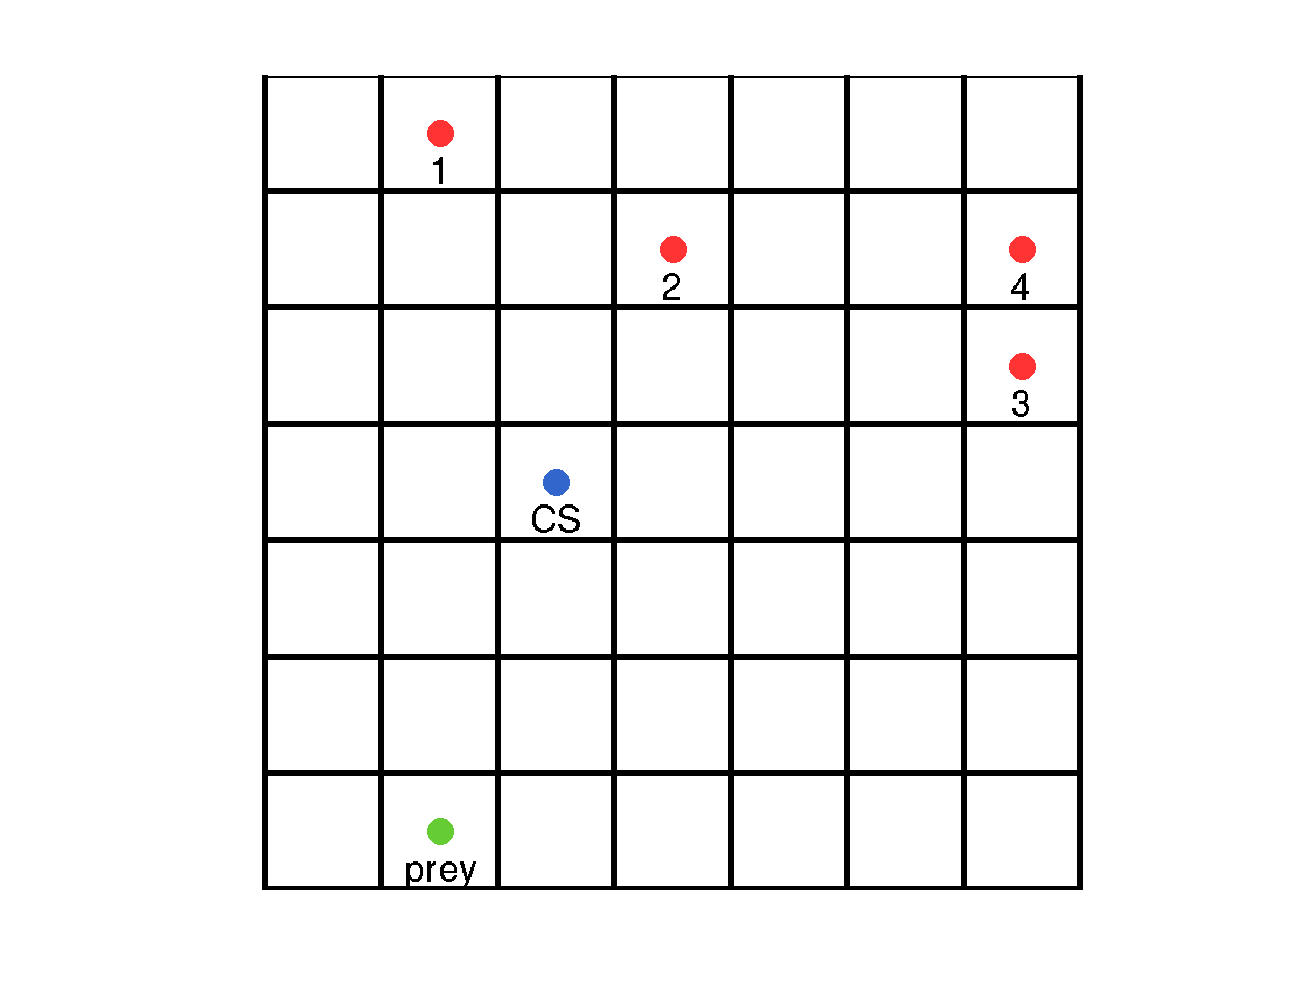
\includegraphics[trim=7cm 3cm 6cm 2cm, clip=true, width=\gridwidth\columnwidth]{plots/visuals/teamConfigRandom.png}%     \caption{A random position}%     \label{subfig:randpos}%   \end{subfigure}%   \begin{subfigure}[b]{0.49\columnwidth}%     \centering%     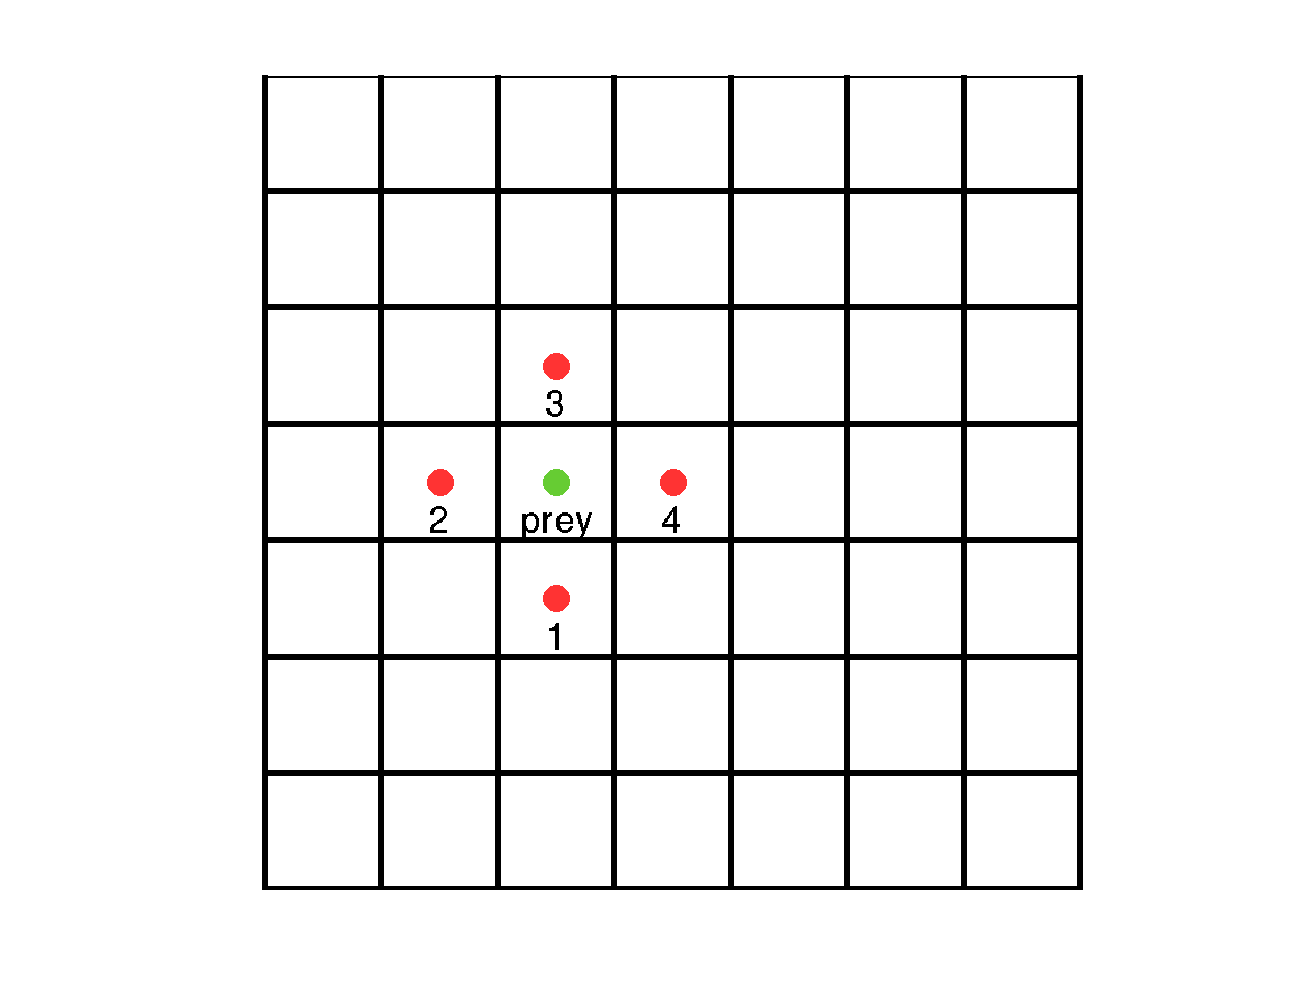
\includegraphics[trim=7cm 3cm 6cm 2cm, clip=true, width=\gridwidth\columnwidth]{plots/visuals/teamConfigCapture.png}%     \caption{A capture position}%     \label{subfig:capturepos}%   \end{subfigure}%   \caption{Start and capture position in the pursuit domain. The green circle is the prey and the red ones are predators. The cell with a blue circle marked with \emph{CS} is the capture state.}%   \label{fig:samplepos}% \end{figure}

In the remainder of this section, we describe how agents plan their actions, as well as the strategy of the predators to lock the prey at the capture state. We first assume predators have full observability of the domain and later remove this ability and describe the communication systems.

\subsection{Notation}

Each position on the grid is called a state $s$, which for convenience is also described as the $(x,y)$ coordinate. For each domain hypothesis $d \in D$, the environment $\env$ is the same, including its dynamic and noise level. A task $\task$ is fully defined by the position of the capture state, denoted $s_C$, that could be any grid cell. The reward function is one when the prey is locked on that state and is zero otherwise. A team configuration $\conf$ describes the role of each agent. For example, $\conf = [N,E,S,W]$ indicates that the first agent is in charge of the North side of the prey, the second one of the East side, etc. The communication protocol $\com$ includes a mapping and a reference (more details are provided in Section~\ref{sec:com}).

\subsection{Action selection method}

To select their actions, all our agents use a two step process. They first assign rewards to states they would like to reach. Then, knowing the full dynamics of the environment, they follow the optimal policy computed using reinforcement learning dynamic programming methods \cite{sutton1998reinforcement}, here value iteration using a discount factor of $0.95$. An agent considers all other agents as static obstacles. %keep this detail for the long version if accepted: If an other agent is in a state whose associated reward is non zero, it is not considered as an obstacle. Indeed, if there is only one state with non zero reward, and if this state is occupied, the agent could never reach such state and the optimal policy would be random -- therefore not optimally progressing towards that state.

When noise is applied, the result of an action can lead to any of the orthogonal directions with equal probability (i.e. if the noise level is $0.2$ and considering no obstacle, taking North action results in the North state with $p=0.8$, the East state with $p=0.1$, and the West state with $p=0.1$). The noise does not affect the ``no move'' action. If an agent moves towards an obstacle, including another agent or the prey, the action fails and the agent stays in its current state.

\subsection{Escaping prey}

The prey tries to escape from its predators by randomly selecting an open neighboring cell to move to. When there is no predator neighboring it, the prey moves randomly. When the prey is surrounded by predators it does not move.

% The prey is trying to escape from its predators but can only see the four states adjacent to its current state. The prey assigns a reward to all neighboring states that are free, and follow the optimal policy to maximize this reward. If the prey is locked by the predators, it selects the ``no move'' action.% As we need to capture the prey in a particular state it is important to have a prey that is trying to escape, such that the predators can guide it towards the capture state. Using a random prey is not well suited because the agent could not influence its behavior.

\subsection{Specialized predators}

The strategy of the team is to guide the prey towards the capture state. Intuitively, two or three predators constrain the prey to move in a specific direction while the remaining predators limit the extent to which the prey can move. For this, some predators will aim for states neighboring the prey, and others will leave one empty cell between them and the prey -- allowing the prey to move in the desired direction. Each predator is specialized to handle one side of the prey (N/S/E/W). For example, the agent in charge of the North side of the prey will target the state directly North of the prey if the prey can reach the capture state faster by going South than by going North. Conversely, if the prey can reach the capture state faster by going North, the North agent will target the state two cells North of the prey -- leaving space for the prey to move towards the capture state by the shortest path. Figure~\ref{fig:capturepos} and \ref{fig:role11} show the targeted team state when chasing the prey in two different conditions.

% The state targeted by each predator depends only of the predator role (N/S/E/W), and the location of the prey. Each predator selects its actions independently of the other predators’ decision.% \begin{figure}%   \centering%   \begin{subfigure}[b]{0.49\columnwidth}%     \centering%     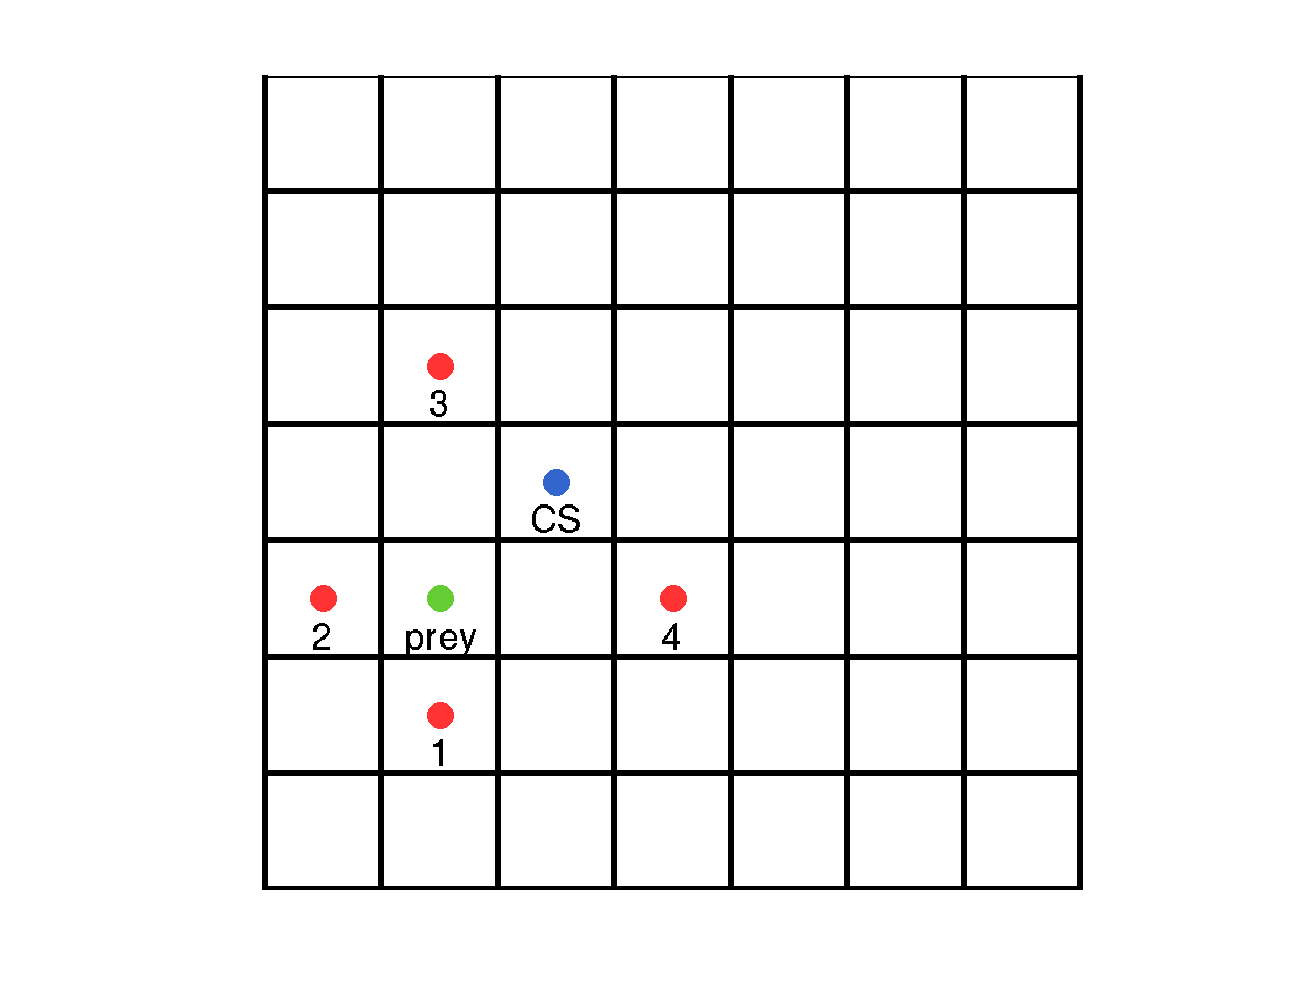
\includegraphics[trim=7cm 3cm 6cm 2cm, clip=true, width=\gridwidth\columnwidth]{plots/visuals/teamConfigApproach.png}%     \caption{The predators chasing the prey to the North-East}%     \label{subfig:rolechasing}%   \end{subfigure}%   \begin{subfigure}[b]{0.49\columnwidth}%     \centering%     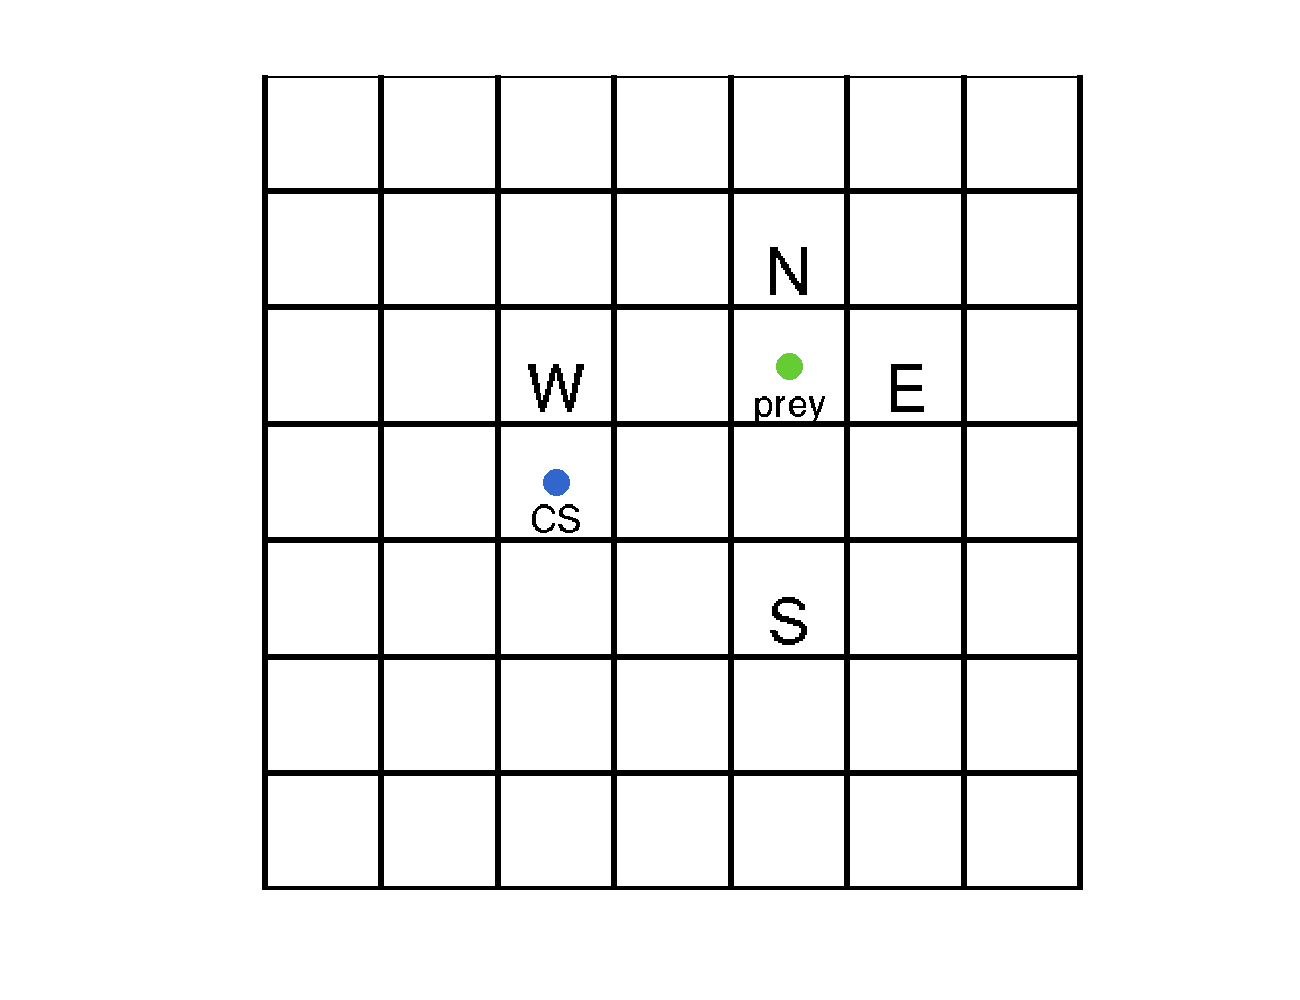
\includegraphics[trim=7cm 3cm 6cm 2cm, clip=true, width=\gridwidth\columnwidth]{plots/visuals/targetStates_33.png}%     \caption{States to target for each predator, chasing South-West}%     \label{subfig:role33}%   \end{subfigure}%   \begin{subfigure}[b]{0.49\columnwidth}%     \centering%     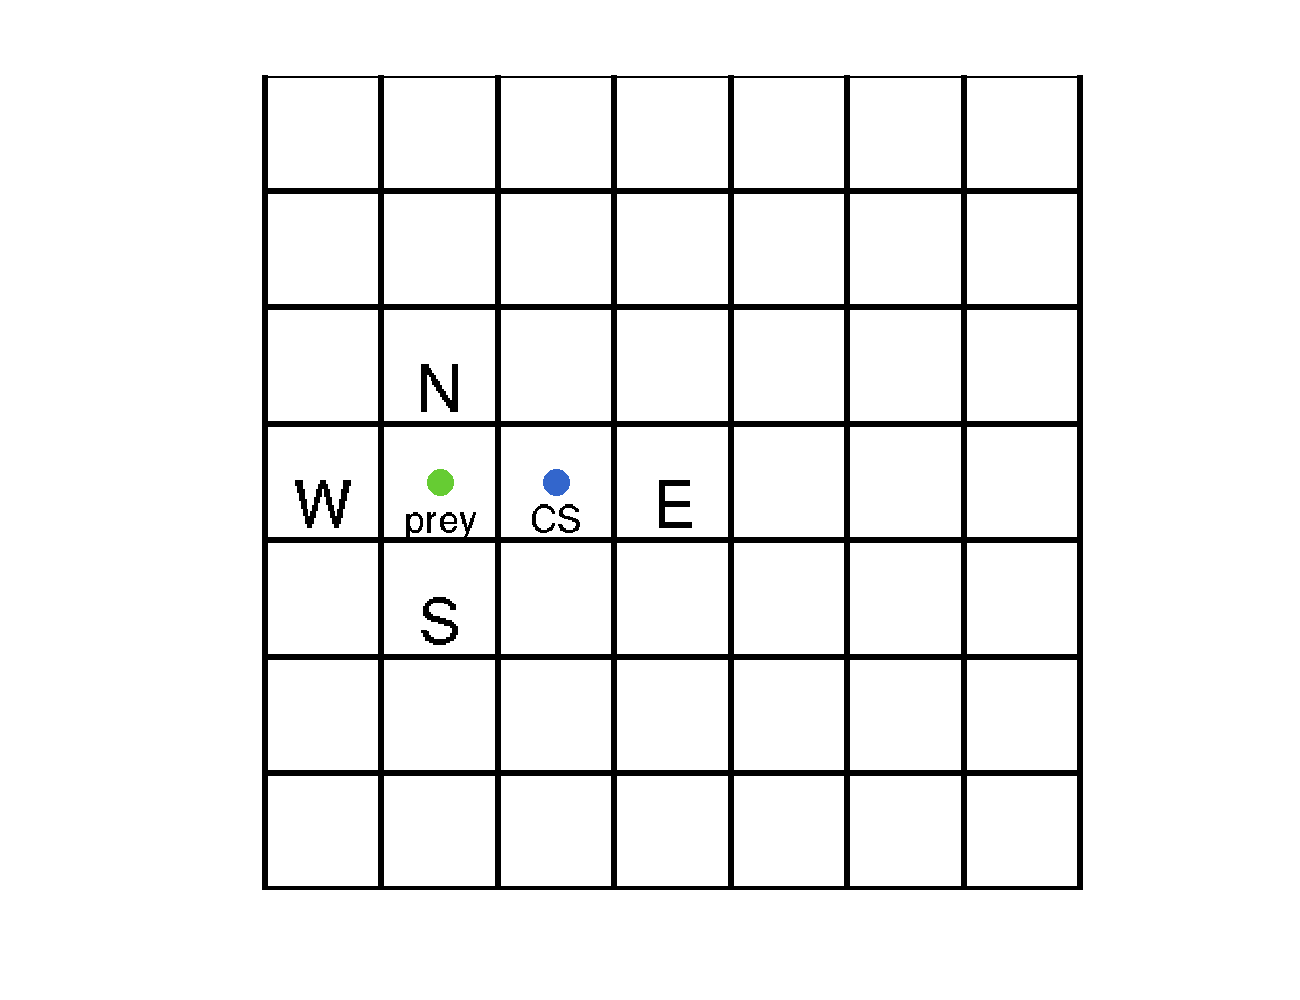
\includegraphics[trim=7cm 3cm 6cm 2cm, clip=true, width=\gridwidth\columnwidth]{plots/visuals/targetStates_11.png}%     \caption{States to target for each predator, chasing East}%     \label{subfig:role11}%   \end{subfigure}%   \begin{subfigure}[b]{0.49\columnwidth}%     \centering%     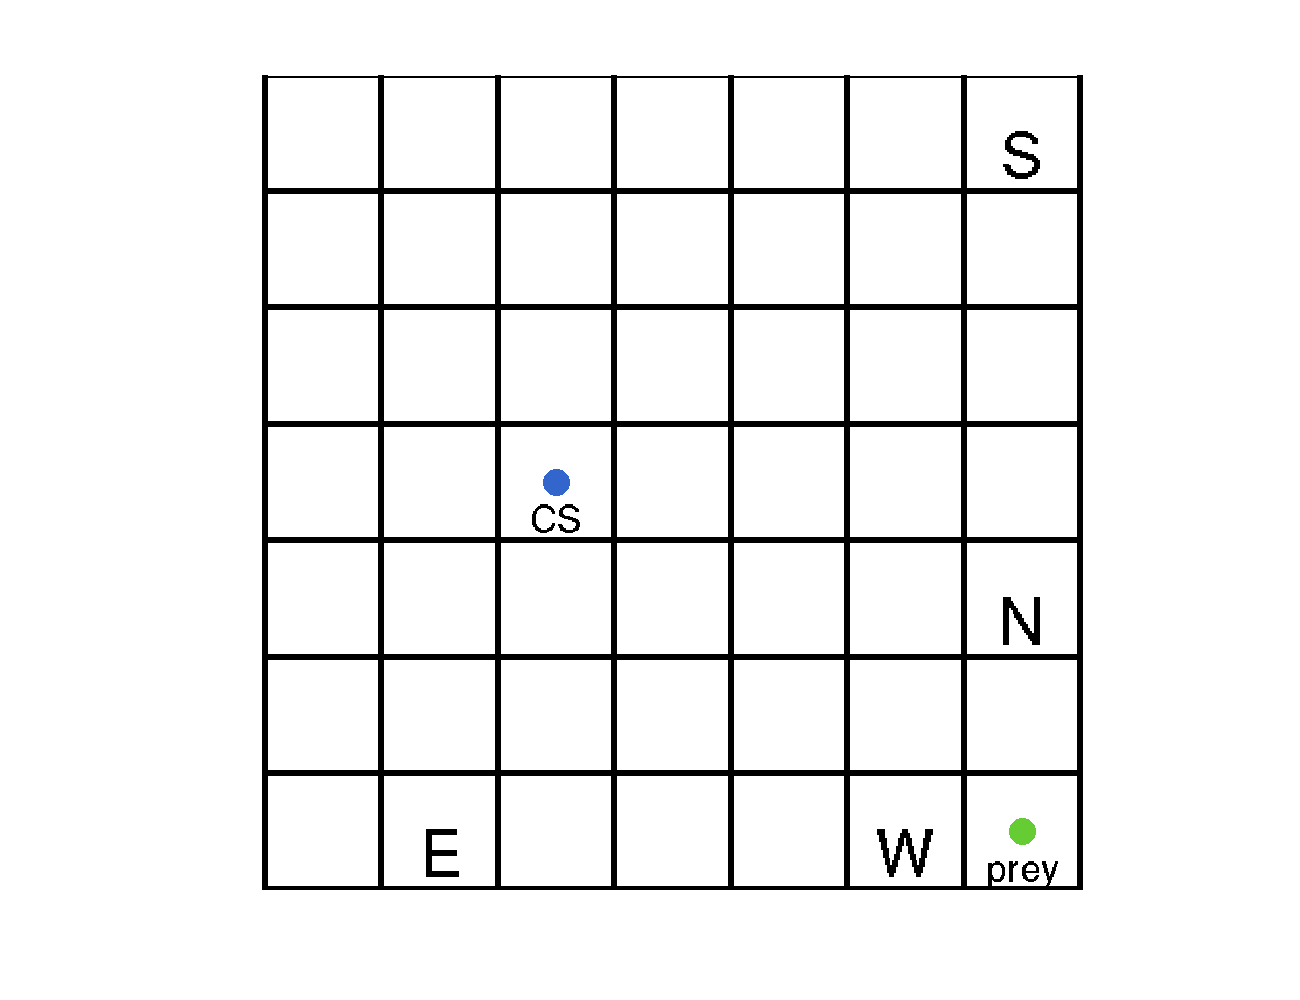
\includegraphics[trim=7cm 3cm 6cm 2cm, clip=true, width=\gridwidth\columnwidth]{plots/visuals/targetStates_43.png}%     \caption{States to target for each predator, chasing South-East}%     \label{subfig:role43}%   \end{subfigure}%   \caption{Examples of states the predators should target to collectively capture the prey. These states depend only on the prey state and the capture state.}%   \label{fig:role}% \end{figure}

If the prey position is known exactly, each predator will aim at only one state, i.e. only one state will have non zero reward for the planning. This corresponds to the situation in Figure~\ref{fig:role11}. The same reasoning can be extended for a probabilistic knowledge of the prey state: for each prey state is associated a target state (as described above), to which we assign as reward the probability of the prey being in the state considered. This is of particular importance for the case of partial observability presented next.

\subsection{Partial observability and communication}
\label{sec:com}

We introduce partial state observability to this domain. We consider predators that can only see the prey if it is one or two steps away from them as illustrated in Figure~\ref{fig:visiblecenter}. The predators can still see each other. As illustrated in Figure~\ref{fig:cmpteam}, partial observability dramatically impacts the team performance. Indeed, if a predator does not see the prey it can only estimate the prey probability to be uniform over the non-observable states. To combat this issue, predators are given the ability to communicate about the prey position. We describe the communication strategy in the following paragraphs.

%One could think of a pursuit domain in tall grass, where the prey is hidden and can only be seen in close range, while the predator are taller and can see each other.% \begin{figure}[htbp!]%   \centering%   \begin{subfigure}[b]{0.49\columnwidth}%     \centering%     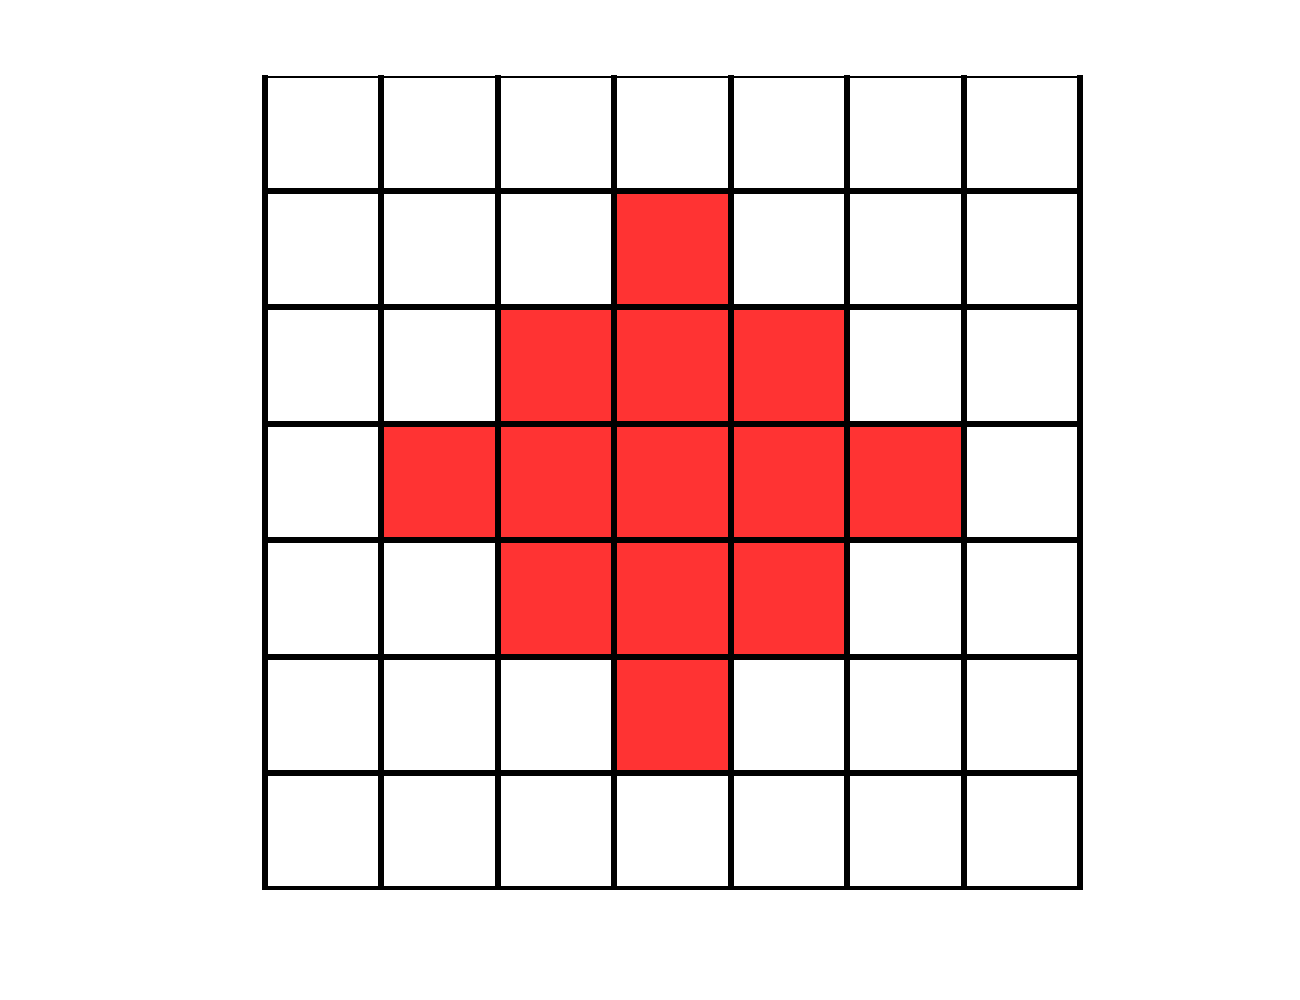
\includegraphics[trim=7cm 3cm 6cm 2cm, clip=true, width=\gridwidth\columnwidth]{plots/visuals/visibleStatesMiddle.png}%     \caption{States observable by a predator located in position (3,3)}%     \label{subfig:visiblecenter}%   \end{subfigure}%   \begin{subfigure}[b]{0.49\columnwidth}%     \centering%     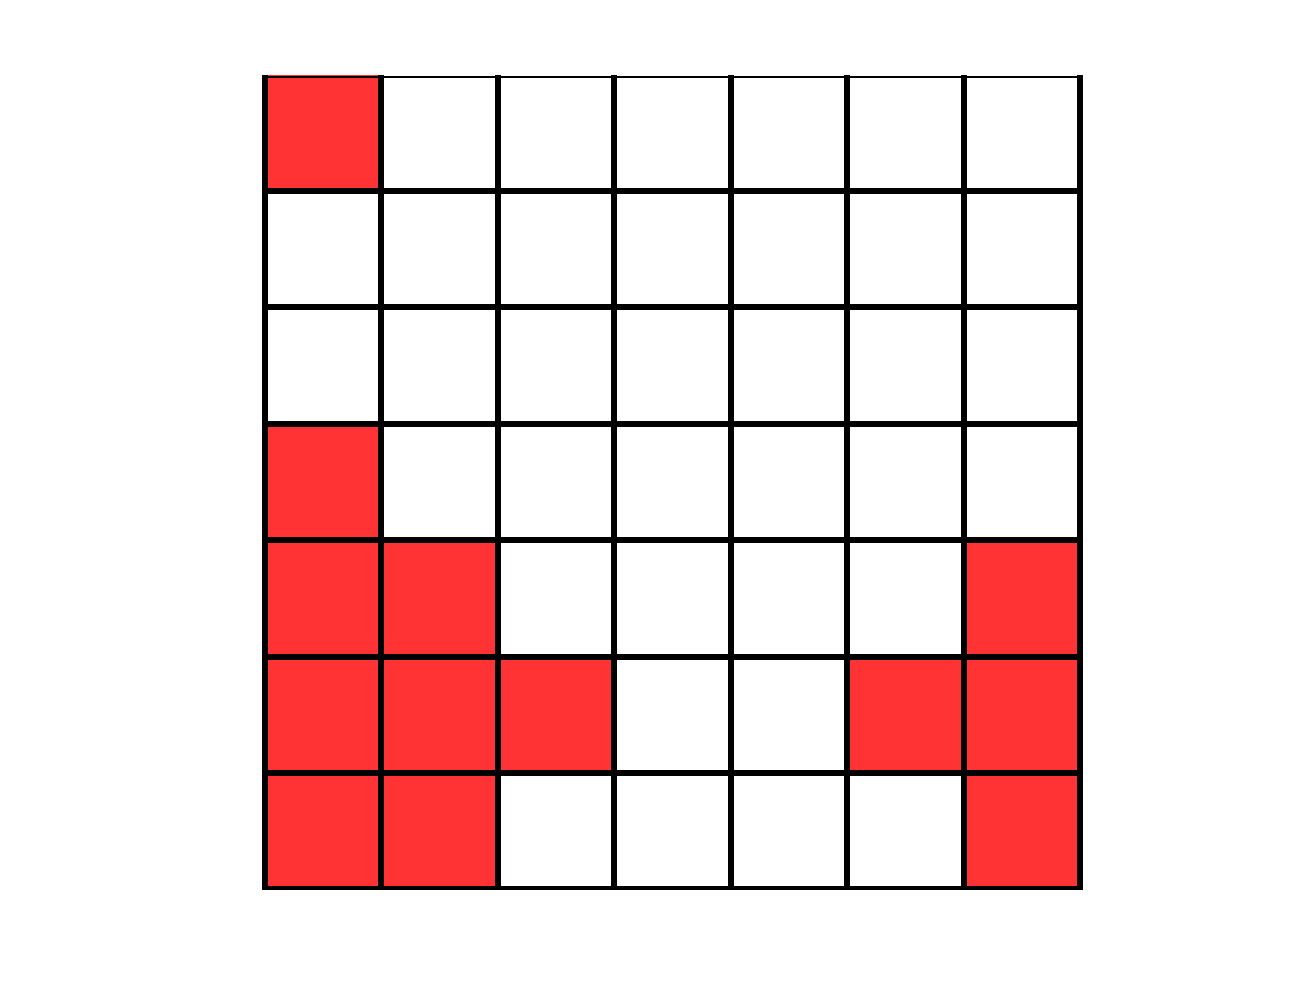
\includegraphics[trim=7cm 3cm 6cm 2cm, clip=true, width=\gridwidth\columnwidth]{plots/visuals/visibleStatesSide.png}%     \caption{States observable by a predator located in position (0,1)}%     \label{subfig:visibleside}%   \end{subfigure}%   \caption{With partial observability, predators can only see two states away from them (shaded red states).}%   \label{fig:visible}% \end{figure}

\subsubsection*{Message encoding} If one agent sees the prey, it can broadcast the position of the prey -- informing all other predators. Therefore, as soon as one agent is in close range with the prey, all other agents are informed, resuming in the full observability case described previously. %This explains the similar performance of the partial observability case with communication as show in Figure~\ref{fig:cmpteam}. Only the cases when no agent sees the prey decrease the performance of such teams.

Each team comes with its own communication protocol $\com$. In some teams, the predators will communicate about the absolute position of the prey in the world, i.e. $(x_{prey},y_{prey})$. In other teams, predators will provide the position of the prey relative to their positions, i.e. $((x_{prey}~-~x_{agent}) ~mod~w, (y_{prey}~-~y_{agent})~mod~h)$. Furthermore, each team has its own ``words'' to designate each of the $n_S$ locations on the grid. In practice, the language is a mapping between a list of symbols and the list of states. In addition, the communication can be noisy such that agents might not always report the correct prey state. There is a uniform probability to refer to a neighboring cell. All predators in a team use the same communication protocol.

\subsubsection*{Message decoding}

Given a set of messages, the prey position is estimated as follows. If the predator can see the prey, it ignores all messages. If it cannot see the prey and there are no messages available, it assigns uniform prey probability to all unobservable states.  If it cannot see the prey and some messages are available, it computes, for each message, the probability of prey position given its knowledge about the noise in the communication, the reference (relative/absolute), and the communication mapping. It then merges this information with the observability area for each agent -- an agent communicates only if it sees the prey. Finally, if several agents communicate, the probabilities of prey state decoded from each messages are combined.% Therefore, if one predator communicates about one prey position it cannot see, the decoder can infer that communication failed (due to noise for example), removing some states from the possible. Finally, if several agents communicate, the probabilities of prey state decoded from each messages are combined. The more agents communicate the better the estimation of the prey state.

For a full team, the probability map of the prey state will never be zero, merging the information from messages of different agents will always be coherent. As we will see in the next section, this might not be the case when the ad hoc agent tries to understand what is going on, which will be valuable to inferring the team communication system.% As described in previous subsection, given a probability map of prey state, each predator computes a reward map given its specific role in the team (N/S/E/W), and selects the optimal action to maximize this reward.
